\section{Articulated System Description}


\subsection{Concepts}

The main idea is to place the description of an articulated system of rigid bodies in the scene graph, so that it can be easily visualized, created and modified. For now, only serial articulated system are considered : it is considered as a hierarchy of 6 dofs solids, starting from a root solid that is fixed by default. (However, it can be animated using \textit{multimapping} approach see\ref{}).
\newline
\newline
The main hypothesis of the Articulated System Description is that the position, velocity and forces (i.e. the mechanical state) of the rigid bodies that are animated with the articulated system are described in the same state with rigid types.

\subsection{Realization}

The description of the articulated system is composed of two parts:
\begin{itemize}
\item The \textbf{articulation centers} provide the point of articulation between two 6D bodies. It is described by its local position on the two bodies: the parent and the child. Its position on the global frame can be deduced from the position in the global frame of the parent.

\begin{figure}[hp]
	\centering
		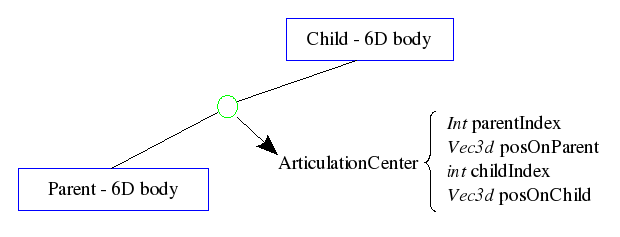
\includegraphics[width=0.6\textwidth]{articulationcenter.png}
	\caption{articulation center}
	\label{articulation center}
\end{figure}

\item Each articulation center has a set of \textbf{articulations} that defines the degrees of freedom of the child on its parent. By default, if no articulation are defined, the position of the child is directly deduced from the position of the parent. Articulation can be translation or rotation and are defined by an axis. Each articulation represent one degree of freedom, and the axis of each articulation are updated sequentially.

\begin{figure}[hp]
	\centering
		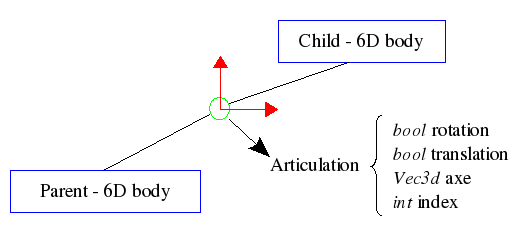
\includegraphics[width=0.5\textwidth]{articulation.png}
	\caption{articulation}
	\label{articulation}
\end{figure}

\end{itemize}


This representation is close to the one use in BVH format. BVH files can be imported in sofa in order to create an Articulated System. An example of an import can be found in the scene \textit{/examples/Components/mapping/ArticulatedSystemMapping\_bvh.scn}.
\newline
\newline
Note that the BVH format also include an animation sequence for each articulation. The values at each frame are re-interpolated in a ArticulatedHierarchyBVHController in order to follow the time step defined in the simulation. This controller provides the position of each articulation in a Vec1 type vector. The motion of the hole articulated system is computed thanks to a mapping described in the following.

\subsubsection{Articulated System Mapping}

The degrees of freedom of the articulated system are given in a Vec1 type vectors containing the position, velocity and force at each articulation.
As the positions of the rigid bodies can be deduced from the position of the articulations, the articulation system can be described in a mapping.
In the scene graph, we obtain:

\begin{figure}[htpb]
	\centering
		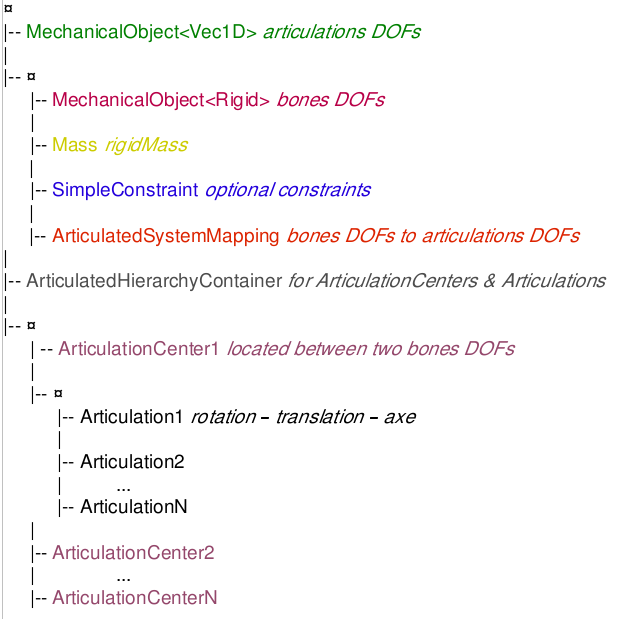
\includegraphics[width=0.5\textwidth]{articulatedsystem_graph}
	\caption{articulated system graph}
\end{figure}

\subsubsection {Example}

The example \textit{/examples/Components/mapping/ArticulatedSystemMapping.scn} shows a basic pendulum :

\begin{code_xml}
<Object type="BruteForceBroadPhase"/>
<Object type="BVHNarrowPhase"/>
<Object type="DefaultContactManager"/>
<Object type="DefaultPipeline"/>
<Object type="ProximityIntersection"/>

<Node>
  <Object type="EulerImplicit" name="cg odesolver" printLog="false"/>
  <Object type="CGLinearSolver" iterations="100" name="linear solver" threshold="1e-20" tolerance="1e-20"/>
  <Object type="MechanicalObject" template="Vec1d" name="Articulations"
          position="0 0 0 0"/>
  <Node>
    <Object type="MechanicalObject" template="Rigid" name="DOFs"
            position="0 0 0  0 0 0 1 
                      1 0 0  0 0 0 1 
                      3 0 0  0 0 0 1 
                      5 0 0  0 0 0 1 
                      7 0 0  0 0 0 1"/>
    <Object type="UniformMass" template="Rigid" name="mass"
            mass="1 1 [1 0 0,0 1 0,0 0 1]"/>
    <Object type="FixedConstraint" template="Rigid" name="fixOrigin"
            indices="0"/>
    <Object type="ArticulatedSystemMapping"/>
  </Node>
  <Object type="ArticulatedHierarchyContainer"/>
  <Node name="articulationCenters">
    <Node name="articulationCenter1">
      <Object type="ArticulationCenter" 
              parentIndex="0" 
              childIndex="1" 
              posOnParent="0 0 0" 
              posOnChild="-1 0 0"/>
      <Node name="articulations">
        <Object type="Articulation" 
                translation="0" 
                rotation="1" 
                rotationAxis="0 0 1" 
                articulationIndex="0"/>
      </Node>
    </Node>
    <Node name="articulationCenter2">
      <Object type="ArticulationCenter" 
              parentIndex="1" 
              childIndex="2" 
              posOnParent="1 0 0" 
              posOnChild="-1 0 0"/>
      <Node name="articulations">
        <Object type="Articulation" 
                translation="0" 
                rotation="1" 
                rotationAxis="0 0 1" 
                articulationIndex="1"/>
      </Node>
    </Node>
    <Node name="articulationCenter3">
      <Object type="ArticulationCenter" 
              parentIndex="2" 
              childIndex="3" 
              posOnParent="1 0 0" 
              posOnChild="-1 0 0"/>
      <Node name="articulations">
        <Object type="Articulation" 
                translation="0" 
                rotation="1" 
                rotationAxis="0 0 1" 
                articulationIndex="2"/>
      </Node>
    </Node>
    <Node name="articulationCenter4">
      <Object type="ArticulationCenter" 
              parentIndex="3" 
              childIndex="4" 
              posOnParent="1 0 0" 
              posOnChild="-1 0 0"/>
      <Node name="articulations">
        <Object type="Articulation" 
                translation="0" 
                rotation="1" 
                rotationAxis="0 0 1" 
                articulationIndex="3"/>
      </Node>
    </Node>
  </Node>
</Node>	

\end{code_xml}

In this example, we have under the first node the components to manage collisions, as usual.
Under the second node, we have :
\begin{itemize}
	\item the solver,
	\item the mechanical object modeling the position of each articulation (4 articulations here),
	\item the container to store all the articulation data.
\end{itemize}

The third node (a child of the previous one) contains the components relative to the articulations :
\begin{itemize}
	\item the mechanical object modeling the independent rigid DOFs (5 rigids here),	
	\item the rigid mass,
	\item a constraint, to fix the first rigid.
	\item the mapping to link the two mechanical objects, as explained before.
\end{itemize}
